% Document settings
\documentclass[11pt]{article}

% Paquetes para usar bien el idioma español
\usepackage[spanish,es-tabla]{babel}
\selectlanguage{spanish}
\usepackage[utf8]{inputenc}

% Paquetes para usar mejores imagenes
\usepackage{graphicx}

% Paquetes para links y tabla de contenidos en el PDF
\usepackage{hyperref}
\hypersetup{colorlinks=true,allcolors=blue}
%\usepackage{hypcap}

% Paquetes para mejores tablas
\usepackage{booktabs}

% Mejor matematica
\usepackage{amsmath}

% Fuentes de las imagenes
\usepackage[absolute,overlay]{textpos}

% Paquete captions
\usepackage[justification=centering,labelformat=empty,labelsep=none]{caption}

% Opciones para ticks
\usepackage{tikz}
\usetikzlibrary{shapes,arrows,positioning}

\tikzstyle{decision} = [diamond, draw, fill=blue!20, text width=4em, text badly centered, node distance=2cm, inner sep=0pt,on grid]
\tikzstyle{block} = [rectangle, draw, fill=blue!20, text width=8em, text centered, rounded corners, minimum height=2em,on grid]
\tikzstyle{line} = [draw, -latex]

% Citas bibliograficas
\usepackage[backend=biber]{biblatex}
\renewcommand{\footnotesize}{\tiny}
\addbibresource{biblio.bib}

% Mejoro las captions
\setbeamertemplate{caption}{\raggedright\insertcaption\par}

\setbeamertemplate{caption}{%
\begin{beamercolorbox}[wd=0.85\paperwidth, sep=.2ex]{block body}\insertcaption%
\end{beamercolorbox}%
}


% Sacar barra de navegacion
\setbeamertemplate{navigation symbols}{}%remove navigation symbols

% Transparencias en items
\setbeamercovered{transparent}

% Estilo de diapositivas
% \usetheme{Boadilla}
\usecolortheme{whale}
\usecolortheme{orchid}

\usepackage{multirow}
\usepackage{longtable}
\setlength\parindent{0pt}

\begin{document}

% Course information
\begin{center}
    {\LARGE SoPI/2 Herramientas de teledetección cuantitativa.}\\
    {\large 2 de septiembre al 4 de noviembre}\\
    {\large 9 a 14 horas, Aula Planta Baja, CONAE}\\
\end{center}
\vspace{10mm}

% Professor information
\begin{center}
\begin{tabular}{ll}
  \multirow{6}{*}{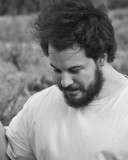
\includegraphics[height=1.25in,width=1in]{pic_fran.png}} &
    \large Francisco Nemiña \\
  & \large \url{fnemina@conae.gov.ar} \\
  & \large \url{https://sopi.conae.gov.ar/aulavirtual} \\
  & \large Av. Paseo Colon 751, 1er piso\\
  & \large Horario de consulta: 9 a 17 horas\\
  & \large +54 11 4331 0074 int. 5699 \\
\end{tabular}
\end{center}
\vspace{5mm}
\begin{center} si $\Delta S_U \ge 0 \Rightarrow$ este documento puede cambiar. \\
\end{center}

% Course details
\textbf {\large \\ Descripción del curso:} El curso busca brindar conceptos
básicos de procesamiento digital de imágenes y extracción de datos cuantitativos
a partir de la utilización de una serie de herramientas que incluyen las etapas
de preprocesamiento, procesamiento y validación de los datos obtenidos. Durante
el curso se trabaja como eje fundamental al concepto de firma espectral desded
un punto de vista del espacio espectral.\\
\textbf {Requisitos:} Haber cursado el curso SoPI I o acreditar conocimientos
equivalentes de teledetección. Es deseable además poseer conocimientos elementales 
sobre físca y matemática al nivel de un graduado en ciencias de la tierra. 
Conocimientos de programación en Python no excluyentes.
\\
\textbf {Nota:} El curso brindará certificado de {\it aprobación}.
\\
% \textbf {Credit Hours:} 3 \\
\\
\textbf {\large Texto:} \emph{Remote Sensing Digital Image Analysis},
5\textsuperscript{th} Edition
\textbf {Autor:} John A. Richards; \\
\textbf {\large Texto:} \emph{Quantitative remote sensing of land surfaces},
\textbf {Autor:} Shunlin Liang;\\
\\
\textbf {\large Objetivos del curso:} \\
Al finalizar el curso, el alumno podr\'a:
\begin{enumerate} \itemsep-0.4em
  \item Familiarizarse con los conceptos de firma espectral.
  \item Poder comprender a un píxel como un objeto vectorial.
  \item Conocer las distintas fuentes de distorsión radiométrica.
  \item Poder realizar operaciones en el espacio espectral.
  \item Poder relacionar indiciones con variables biofisicas.
  \item Comprender el concepto de dimensionalidad de un espacio.
  \item Poder realizar clasificaciones supervisadas y no supervisadas.
  \item Comprender la necesidad de realizar validaciones sobre los datos
      obtenidos.
  \item Conocer como realizar validaciones desde el punto de vista operativo.
  \item Comprender los fundamentos matemáticos de estos procesos.
\end{enumerate}
\newpage
% I recommend using \newpage here if necessary
\textbf {\large Puntajes de la nota:} \\
\begin{center}
\begin{tabular}{lc}
    \emph{Actividad} & \emph{Puntaje} \\
    \toprule
Cuestionarios & 5 cada uno\\
Trabajos práctico & 10 cada uno \\
Trabajo final & 40 \\
Respuestas en el foro & 1 cada una\\
Asistencia & 2 cada clase \\
\end{tabular} \\
\end{center}
\textbf {\large Distribuci\'on de notas:} \\\\
\begin{center}
\begin{tabular}{cc}
    \emph{Puntaje} & \emph{Nota}\\
    \toprule
    170 a 166 & 10 \\ 165 a 156 & 9 \\
    155 a 116 & 8  \\ 115 a 105 & 7 \\
    105 a 101 & 6  \\ 100 a   0 & No aprobó
\end{tabular} \\
\end{center}
% Course Policies. These are just examples, modify to your liking.
\textbf {\large Politicas del curso:}
\begin{itemize}
	\item \textbf {General}
		\begin{itemize}
			\item Los cuestionarios se completaran de forma online.
            \item Los trabajos prácticos serán enviados en forma online.
			\item Los cuestionarios se podrán rendir \textbf{una} sola vez.
		\end{itemize}
	\item \textbf {Cuestionarios y trabajo final}
		\begin{itemize}
			\item Los estudiantes deberán trabajar por su cuenta.
			\item No se aceptaran los cuestionarios completados fuera de fecha.
		\end{itemize}
\end{itemize}

% Course Outline
\newpage
\textbf {\large Cronograma tentativo}:

\begin{longtable}[h!]{| c | c | }
%\normalsize % The size of the table text can be changed depending on content. Remove if desired.
%\begin{tabular}{ | c | c | }
\toprule
\textbf{Día} & \textbf{Contenido} \\

\midrule
4/septiembre & \begin{minipage}{.65\textwidth}
\begin{itemize} 
    \vspace{1mm}
\item Teoría: Introducción al curso. Repaso de álgebra lineal. Vectores y matrices. Operaciones con vectores y matrices. Espacios vectoriales. Transformaciones lineales. Resolución de sistemas de sistemas de ecuaciones. Diagonalización. Autovalores y autovectores.
	  \item Práctica: Operaciones matriciales en python. Sumas y diagonalización. Problema de inversión. 
	\item Lecturas: Richards - Capítulo 3 y apéndice C. 
    \vspace{1mm}
\end{itemize}
\end{minipage} \\

\midrule
9/septiembre & \begin{minipage}{.65\textwidth}
\begin{itemize} 
    \vspace{1mm}
  \item Teoría: Definición de magnitudes físicas. Radiancia. Irradiancia. Reflectancia bidireccional. Construcción de firmas espectrales. Características de un sensor. Firma espectral del agua, suelo y vegetación. Mezcla y desmezcla de firmas espectrales.
  \item Práctica: Familiarización con la interfaz de SoPI\@. Extracción y ploteo de firmas espectrales. Interpretación de firmas espectrales. Desmezcla espectral.
	\item Lecturas: Richards - Capítulo 1. Liang - Capítulo 1.
    \vspace{1mm}
\end{itemize}
\end{minipage} \\
\midrule
16/septiembre & \begin{minipage}{.65\textwidth}
\begin{itemize} 
    \vspace{1mm}
	\item Teoría: El sol como fuente de energía. Magnitudes. Radiancia y reflectancia. Magnitudes a tope de la atmósfera. Cálculo de irradiancias solares por banda. Convolución espectral. Corrección por ángulo solar. Ecuación de transferencia radiativa. Soluciones cerradas. Aproximaciones. Dispersión y absorción en la atmosfera terrestre. Bandas de absorción. Dispersión por Rayleigh. Corrección por substracción de pixel obscuro. Errores por omisión de correcciones.
  \item Práctica: Corrección de DN a reflectancia a tope de la atmósfera (TOA). Corrección por sustracción de pixel oscuro. Corrección con 6S. Comparación de firmas espectrales de imágenes corregidas y no corregidas.
	\item Lecturas: Richards - Capítulo 2. Mahiny, Abdolrassoul S., and Brian J.
        Turner. "A comparison of four common atmospheric correction methods."
        Photogrammetric Engineering \& Remote Sensing 73.4 (2007): 361-368.
    \vspace{1mm}
\end{itemize}
\end{minipage} \\

\midrule
23/septiembre & \begin{minipage}{.65\textwidth}
\begin{itemize} 
    \vspace{1mm}
	\item Teoría: Imágenes como vectores. Dimensionalidad. Selección de bandas en función del problema. Reducción de dimensionalidad. Índices. Construcción de índices a partir de una firma espectral. Relación entre índices y variables biofísicas. Índice de vegetación. Índice de vegetación normalizado. Otros índices de vegetación.
  \item Práctica: Cálculo y construcción de imágenes a partir de índices. Construcción de firmas fenológicas a partir del NDVI.
	\item Lecturas: Liang - Capítulo 8.
    \vspace{1mm}
\end{itemize}
\end{minipage} \\


\midrule
30/septiembre & \begin{minipage}{.65\textwidth}
\begin{itemize} 
    \vspace{1mm}
	\item Teoría: Transformaciones como rotaciones. Cálculo por componentes principales. Transformada tasseled-cap. Aplicaciones de cálculo de componentes principales a imágenes multibanda y series temporales de imágenes
  \item Práctica: Calculo de componentes principales sobre imágenes sobre apilados de imágenes multiespectrales y series temporales de índices. Transformada tasseled-cap. Interpretación de las bandas obtenidas por el análisis de componentes principales.
	\item Lecturas: Richards - Capítulo 6. 
    \vspace{1mm}
\end{itemize}
\end{minipage} \\

\midrule
7/octubre & \begin{minipage}{.65\textwidth}
    \vspace{1mm}
\emph{Clase de consulta.}
    \vspace{1mm}
\end{minipage} \\

\midrule
14/octubre & \begin{minipage}{.65\textwidth}
\begin{itemize} 
    \vspace{1mm}
	\item Teoría: Métodos de clasificaciones supervisadas. Clasificación por máxima verosimilitud, distancia mínima y paralelepípedos. Ventajas y desventajas de cada algoritmo. Selección de clases iniciales. Unicidad de la clasificación. Efecto Hughes. Técnicas de post-clasificación.
	\item Práctica: Clasificación supervisada para la generación de mapas de coberturas. Métodos de selección de clases de entrenamiento. Firmas espectrales para las clases iniciales. Comparación entre métodos supervisados y no supervisados. Máscaras.
	\item Lecturas: Richards - Capítulo 8.
    \vspace{1mm}
\end{itemize}
\end{minipage} \\

\midrule
21/octubre & \begin{minipage}{.65\textwidth}
\begin{itemize}
    \vspace{1mm}
	\item Teoría: Transformación de clases espectrales a clases de información. Extracción de datos cuantitativos. Métodos de clasificaciones no supervisadas, clustering, algoritmo k-means, convergencia y problemas del algoritmo, selección inicial de clases. Costo computacional.
  \item Práctica: Clasificación no supervisada para la generación de mapas de coberturas. Clasificación por algoritmo k-means y fusión de clases.
	\item Lecturas: Richards - Capítulo 9.
    \vspace{1mm}
\end{itemize}
\end{minipage} \\

\midrule
28/octubre & \begin{minipage}{.65\textwidth}
\begin{itemize}
    \vspace{1mm}
	\item Teoría: Precisión de un mapa, toma de puntos en el terreno, diseño de muestreos, error en la precisión de la determinación de puntos en el terreno, construcción de matriz de confusión, precisión total, del productor y del usuario, técnicas básicas de análisis, índices.
  \item Práctica: Cálculo de matrices de confusión para clasificaciones supervisadas y no supervisadas. Comparación entre las clasificaciones supervisadas y no supervisadas a partir de la matriz de confusión. Ventajas y desventajas de cada método.
	\item Lecturas: Olofsson, Pontus, et al. "Good practices for estimating area and assessing accuracy of land change." Remote Sensing of Environment 148 (2014): 42-57.
    \vspace{1mm}
\end{itemize}
\end{minipage} \\

\midrule
    \vspace{1mm}
4/noviembre & \begin{minipage}{.65\textwidth}
\emph{Clase de consulta.}
\end{minipage} \\
\bottomrule

%\end{tabular}
\end{longtable}

\end{document}
